% \begin{figure}[h]
% 	\centering
% 	\subfig[.43]{PlanarConcept.png}{.2}{planar}
% 	\begin{subfigure}{0.1\textwidth}  
% 		\centering 
% 		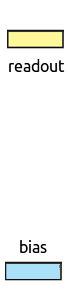
\includegraphics[height=.2\textheight]{LegendConcept.png}
% 		\vspace*{19pt}
% 	\end{subfigure}
% 	\subfig[.43]{3DConcept.png}{.2}{3D}
% 	\caption{Comparison of the planar and the 3D detector concepts}
% 	\label{3d1}
% \end{figure}
% The radiation damage created by the \ac{HL-LHC} will become a big challenge for the innermost tracking detectors. 
After large irradiation, all detector materials become trap limited with a \ac{MFP} below \SI{75}{\micro\meter}. The concept of a 3D detector is a possible way to reduce the drift distance below the this \ac{MFP}. More details about the fabrication and the functionality can be found in \cite{3D}, \cite{parker}.\par
%%%%%%%%%%%%%%%%%%%%%%% CONCEPT %%%%%%%%%%%%%%%%%%%%%%%%%%%
% Its basic principle is shown in figure \vref{3d1}: In a planer detector the readout and bias electrodes are brought onto the front and back side of the sensor with a thickness $\Updelta$. The resulting drift distance L of the charge carriers is of the order of $\Updelta$. In the 3D detector the electrodes are put inside of the detector material so that the \acp{MIP} can travel the same distance $\Updelta$ in the material and therefore create the same amount charge carriers but L is heavily reduced. In case of diamond these electrode columns are drilled with a \SI{800}{\nano\meter} femtosecond laser which converts the diamond into a resistive mixture of carbon phases.\\
%%%%%%%%%%%%%%%%%%%%%%% MULTI %%%%%%%%%%%%%%%%%%%%%%%%%%%%%
In 2015 the first detector was built out of a \pcvd diamond sensor which had 3D readout 
\wrapfigcl{3DMultiResult.png}{.35}{Pulse height of the 3D multi detector}{3d2}
with ganged readout columns as well as a strip metallisation on the same sensor. The thickness of sensor was \SI{\sim500}{\micro\meter} and the 3D cells had a size of \SI{150x150}{\micro\meter}. At this time the column production efficiency was about \SI{92}{\%} \cite{felix}.
% Its square cells are clearly visible and
The mean of the measured pulse height is \SI{13500}{e} which is much higher than \SI{6900}{e} in the strip detector on the same diamond. The strip signal equates to a \ac{CCD} of \SI{192}{\micro\meter} whereas the charge in the 3D would have a \ac{CCD} in a planar detector of \SIrange{350}{375}{\micro\meter} which effectively means that more than \SI{75}{\%} of the created charge was collected for the first time in a \pcvd diamond. The corresponding pulse height distributions are shown in Figure \vref{3d2}. This detector was already a success by showing a working 3D diamond detector. \par
%%%%%%%%%%%%%%%%%%%%%%% FULL 3D %%%%%%%%%%%%%%%%%%%%%%%%%%%
In 2016 a full 3D detector was constructed with dramatic improvements. The number of cells was scaled up from 99 to 1188, the cell size was reduced to to \SI{100x100}{\micro\meter} and the column production efficiency was increased to \SI{99}{\%}. The analysis of this device is still in progress but the first results already show charge in the entire area of the detector and it has the largest charge collection in \pcvd with over \SI{85}{\%} in a contiguous region.\par
%%%%%%%%%%%%%%%%%%%%%%% 3D PIXEL %%%%%%%%%%%%%%%%%%%%%%%%%%
Finally at the end of 2016 the first \pcvd 3D sensor with pixel readout which was metallised and then bump bonded to a CMS pixel \ac{ROC} PSI46digV2.1respin \cite{kornmayer}. The chip was then tuned to a global pixel threshold of \SI{1500}{e}. The preliminary beam test results show an efficiency of \SI{98.5}{\%}. This value is close to the efficiency of a silicon pixel of \SI{99.3}{\%} which was tested in parallel. Compared to the silicon the 3D pixel detector has a relative efficiency of \SI{99.2}{\%}. The loss of \SI{0.8}{\%} is believed to originate from the low field regions between the electrodes.